
\chapter*{User Accounts, Access, Data Locations}
% G. Bakos contacted former postdoc Miguel de Val-Borro (now employed by NASA) to create an account for me on the relevant servers. I am now in the hatuser and hatpipebin groups. Bakos says we will discuss later whether I need an account on TRAC (e.g. hatreduc), but not for the time being.

VPN into UW Network then connect to server:
\begin{minted}{bash}
    smb://research.drive.wisc.edu/rmathieu
\end{minted}

Discuss the K2 mosaic pipeline here

% The K2 pipeline is installed on phs3 and there is some raw data available under /nfs/phs3/ar1/ (91\% full at this time). As of 09/16/2015, Field 0 data were moved by Chelsea to phs11 for image subtraction. I now pretty much only use phs11.

\section*{Raw Data Location}
% Chelsea downloaded K2 data from Campaigns 0, 1, and 2. I really only need to use Campaign 0 data at this point in time.
% \begin{itemize}
% \item \textbf{Campaign 0 -- data is under reduced on server phs11 (image subtraction necessary)}
% \item Campaign 1 -- fully reduced light curve on server phs3 
% \item Campaign 2 -- under reduced on server phs11 (image subtraction necessary)
% \end{itemize}

% Directories used by Chelsea:
% \begin{itemize}
% \item  phs3 $\rightarrow$ /nfs/phs3/ar1 (close to full)
% \item phs11 $\rightarrow$ /nfs/phs11/ar0
% \item \textcolor{blue}{The data I want are located on phs11 in the subdirectory\\ \textbf{/S/PROJ/hatuser/2015\_K2/K2\_0} (read only files)}
% \end{itemize}

\subsection*{Data Reduction Location}

\section*{Guidance from Melinda}
\subsection*{Basics}

\subsection*{The K2 Field 0 Data Set}
Kepler original campaign channel 81 contains NGC 6791. All the availble raw fits files are available at \textbf{~/rmathieu/NGC6791}. I do not use these raw files for anything as k2-mosaic downloads the data as a part of the stitching process. 
'''
For each quarter in each of the four years we have to do 

\begin{minted}{bash}
\$ k2mosaic tpflist Q[N] [CHN] \> tpflist.txt
\$ k2mosaic mosaic tpflist.txt 
\end{minted}

if you get stopped add --cadence #####..##### between mosaic and tpf 


e.g. \$ k2mosaic mosx   aic 30771..33935 tpflist.txt 
\\ \\
Channels are 81, 53, 29, 1 so this has to occur for \\
Q4, Q8, Q12, Q16 for channel 81 \\
Q3, Q7, Q11, Q15 for channel 53 or 1 \\
Q2, Q6, Q10, Q14 for channel 29 \\ 
Q1, Q5, Q9,  Q13, Q17 for channel 1 or 53 (Q1 is only 34 days, Q0 is 9 days) \\

We start with just channel 81 for our initial round of analysis 

\subsubsection{90$^\circ$ Roll}
"The Kepler spacecraft rotates by 90o approximately every 93 days to keep its solar arrays directed towards the Sun (Haas et al. 2010). The first 10 days of science data obtained as the last activity during commissioning is referred to as Q0. There were 34 days of observations during Q1 following Q0 at the same orientation. Subsequent quarters are referred to as Q2, Q3, etc., and these each contain 93 days of observations. Transit searches are performed nominally every three months after each quarterly data set has been downlinked to the ground and processed from CAL through PDC" KSCI-19081-001 Data Processing Handbook \S8


\subsection*{Stitching Field with \texttt{k2-mosaic}}
Used the k2-mosaic \texttt{http://k2mosaic.geert.io/} package to create *.fits files of all available cadence of channel 81

\subsection*{Make the \texttt{fistar} Files}
The \textbf{.fistar} file is really just a simple text file with the sources extracted. 
To create these files, I used the \textttt{fistar} command in the file containing the fits files:

\\\texttt{for i in *.fits; do fistar "\$i" -o \$(echo \$i | sed s/fits/fistar/)  -s flux --comment 
--model elliptic --flux-threshold 1000 --algorithm uplink --iterations symmetric=2,general=1 
--format id,x,y,bg,amp,s,d,k,flux,s/n,cmax,fwhm,npix,sigma,delta 
--mag-flux 16.62,30; done}\\
I now do this in the python script

\subsection*{??\texttt{grmatch}}
Make sure that the output is sane by checking  \textbf{Residual} and \textbf{Unitarity} and \textbf{Ratio}.

\subsection*{Transform to \texttt{fitrans}}
\texttt{fitrans *.fits -k --input-transformation *.itrans --reverse -o *-xtrns.fits}.\\ 
These new output fits files have been shifted to our master coordinate reference frame and may be stacked. It is important to make sure that they look as though they have been shifted appropriately. I do this by creating .png image files from the .fits files and then stringing them together to a quick movie.

\subsection*{Mean Photo Reference Frame from \sout{\texttt{ficombine}}}
Using \texttt{ficombine} fails because the input list it too long so I do this with \texttt{numpy}.

The desired command is given here:\\
\texttt{ficombine *xtrns.fits --mode mean -o photref.fits}
\begin{center}
\includegraphics[width=0.5\textwidth]{meanField.png}
\end{center}

\subsubsubsection*{Using \texttt{ficonv} + \texttt{ficombine}}
"A better way to stack the images is to use \texttt{ficonv}. This method, however, builds upon the prior, as it will use the outputted photoref file described in the previous section. 
To start the ficonv+ficombine process, I need to generate something called a \texttt{region file}. The region file gives \texttt{ficonv} an idea of the position of bright stars on the frame to have a good initial start.
The way to go about doing this is to use the script regslct.py, which I have edited and renamed as \texttt{melinda\_regslct.py}.
This script has a single function in it and takes in a \texttt{fistar} file. Joel recommends using the highest focused image, however with Kepler it is unlikely that the focus will change much. To determine the sharpest focused image, check the median value for the \textbf{s} parameter in the \texttt{.fistar} files, which is the inverse variance of the star.
Using the smallest value of the FWHM or the largest \textbf{s} value instead?\\ \\ 
Double check the following values in the script: \textbf{colflux},  \textbf{xsize}, and \textbf{ysize}.
\begin{center}
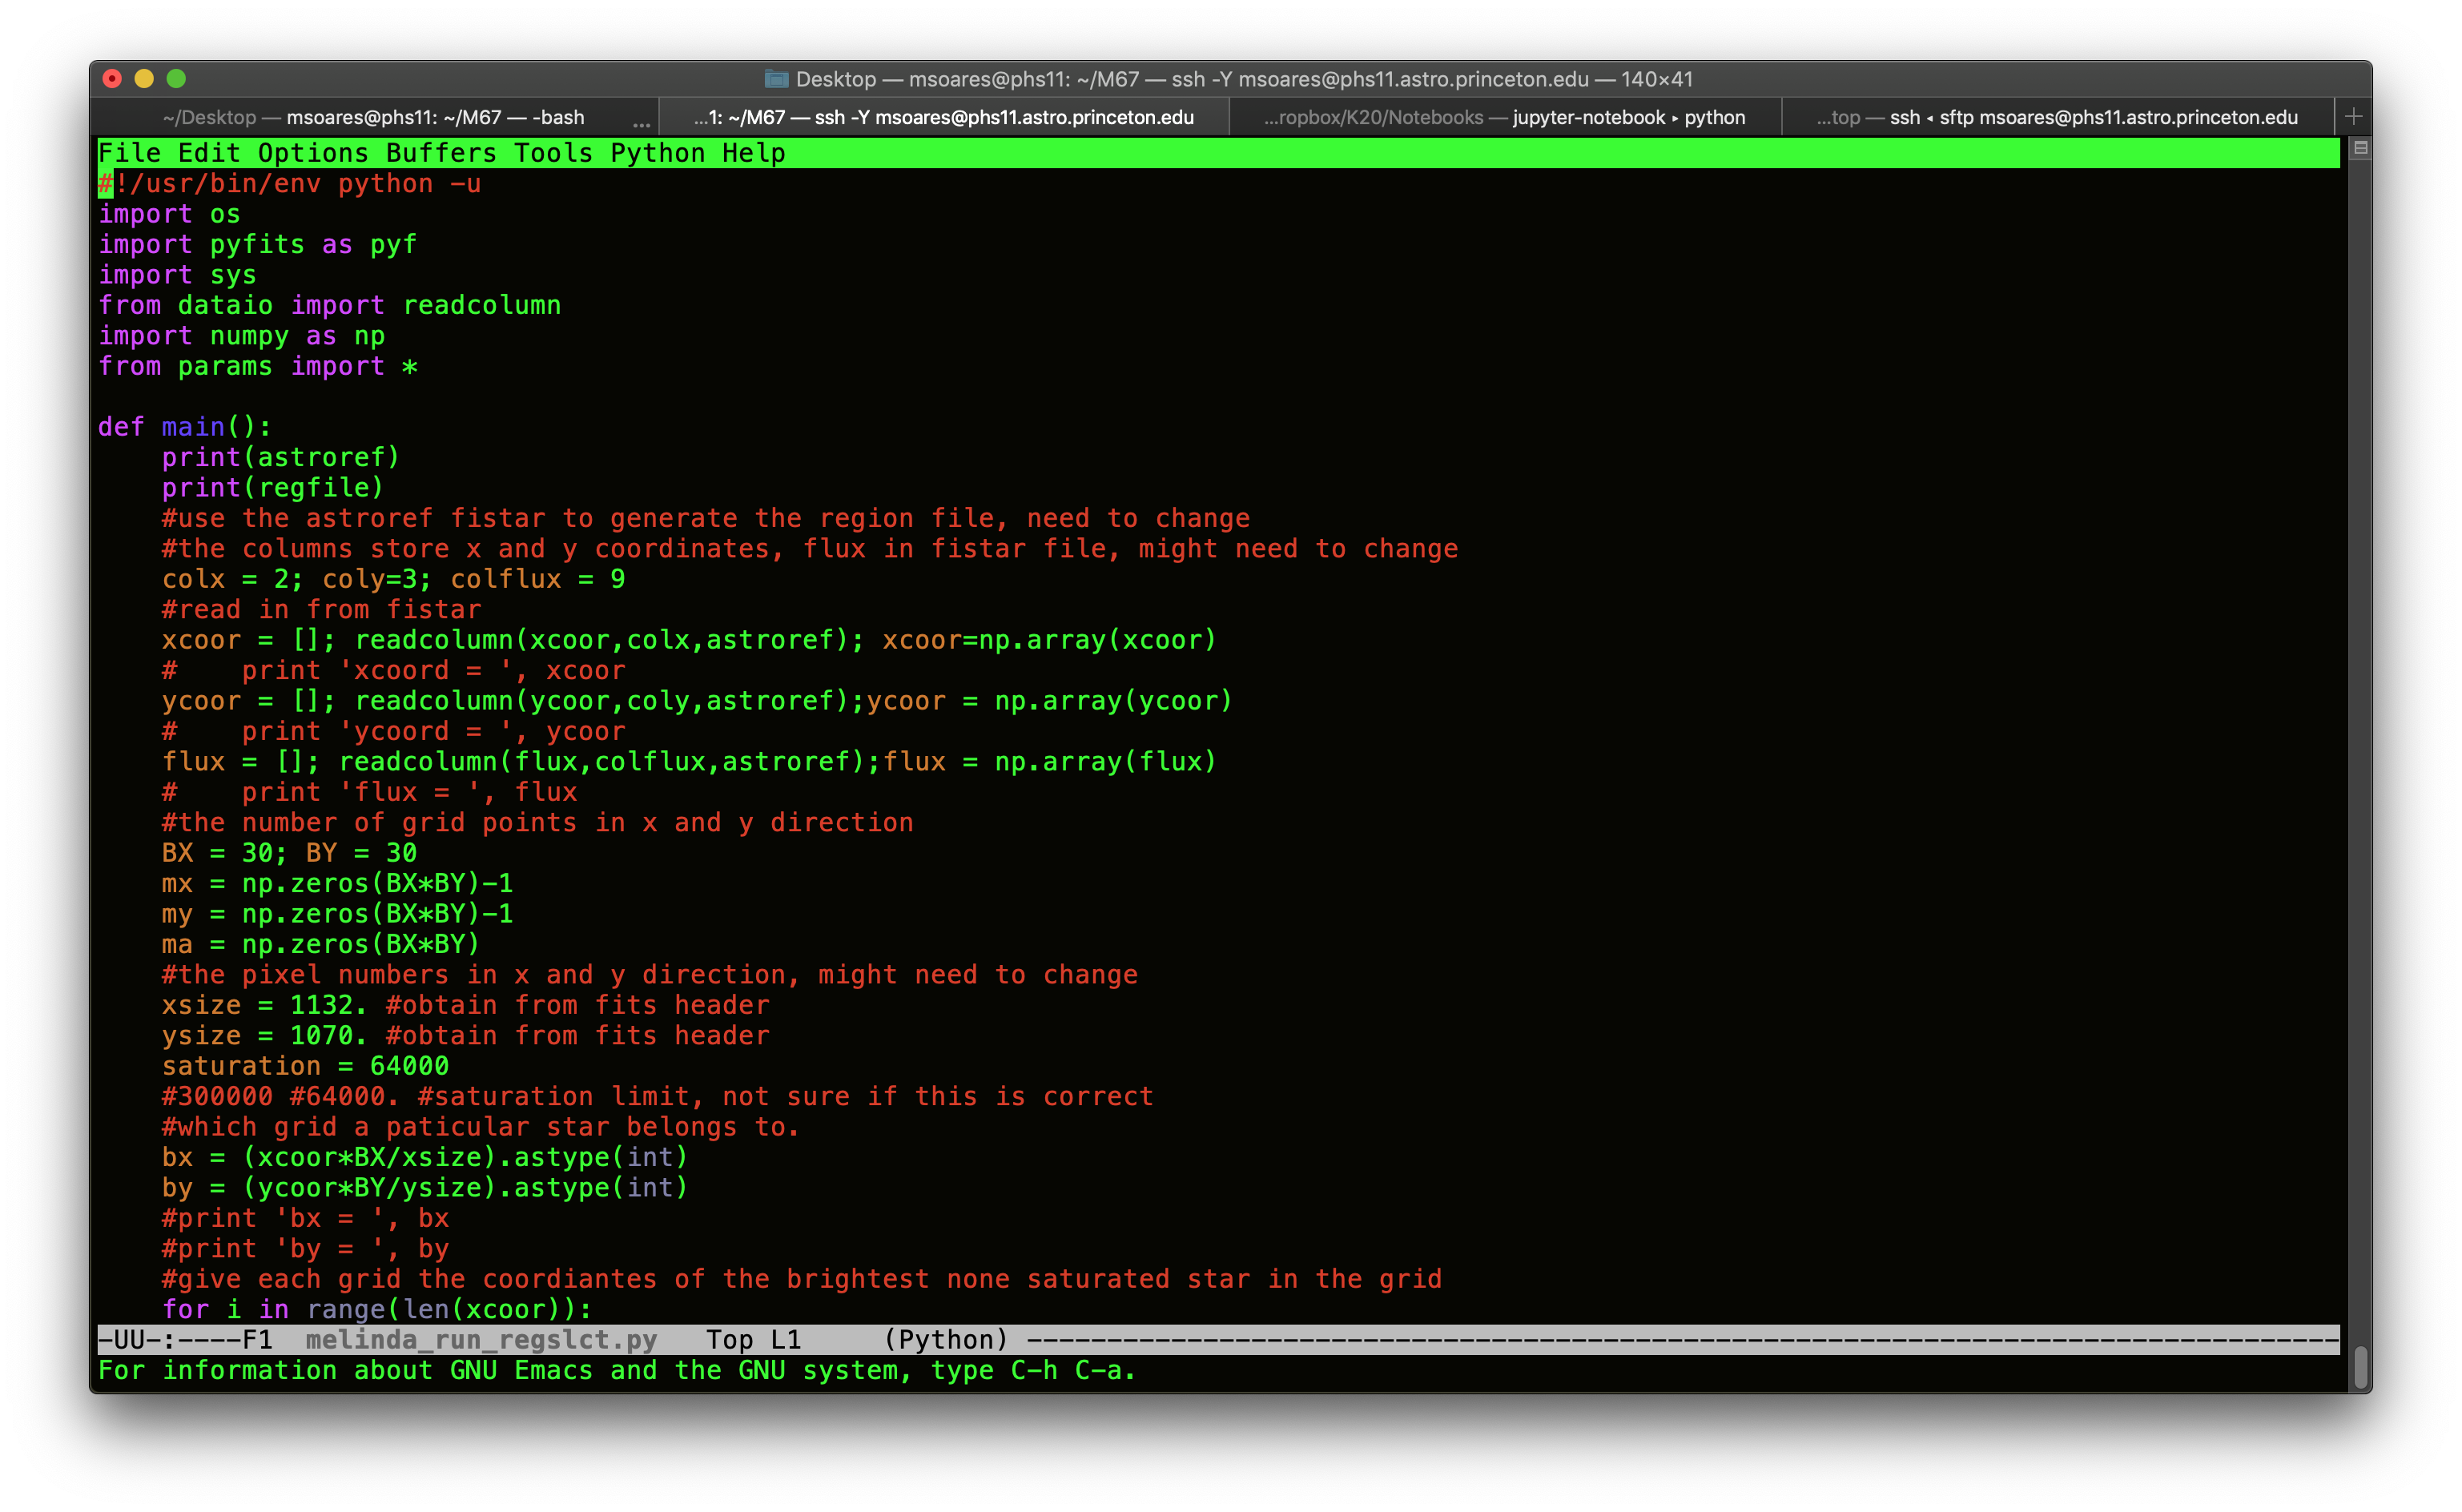
\includegraphics[width=0.8\textwidth]{regslct.png}
\end{center}
\begin{center}
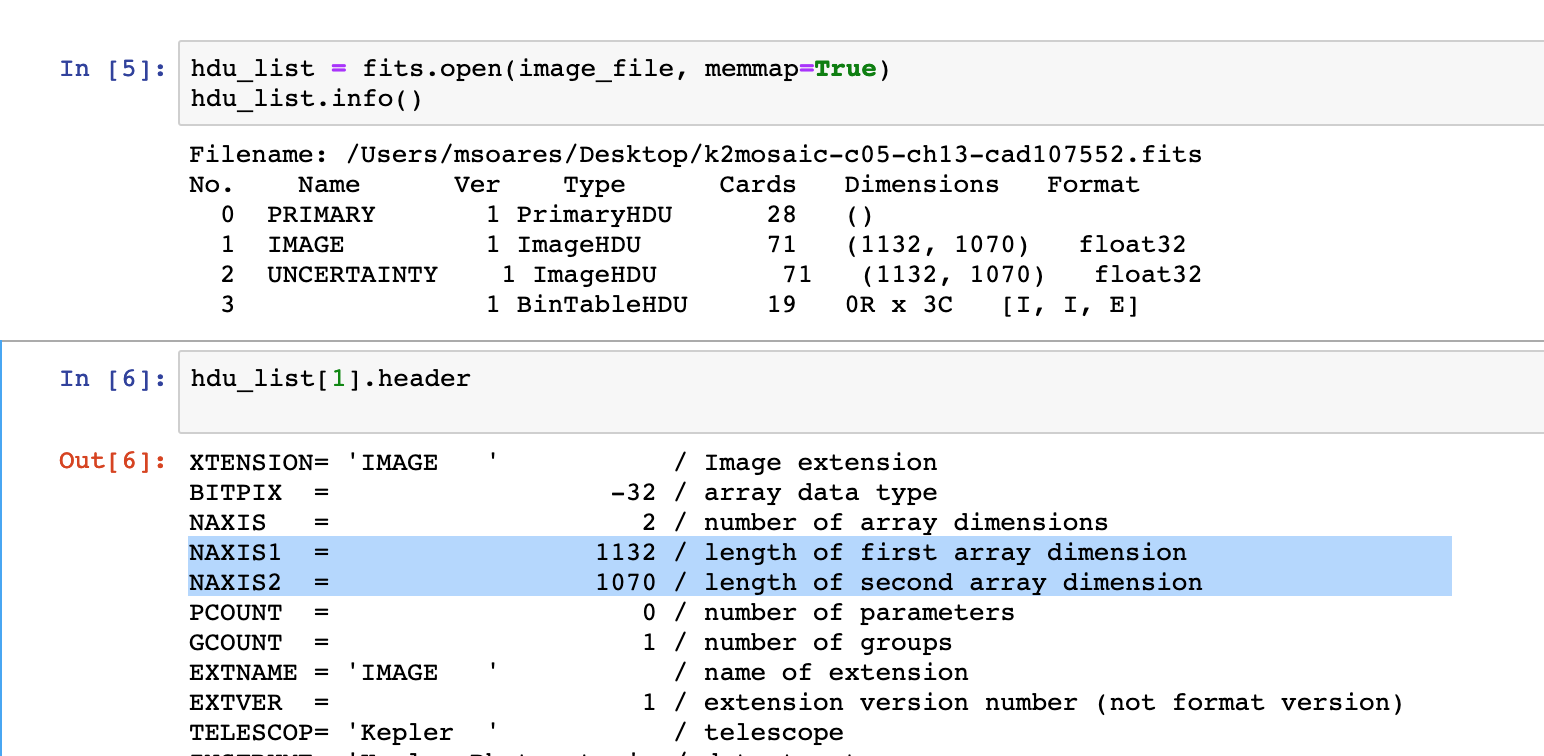
\includegraphics[width=0.8\textwidth]{header.png}
\end{center}

\subsubsection*{? \texttt{ficonv}}
Takes a \texttt{.itrans}, \texttt{*xtrns.fits}, and a \texttt{region} file to run. I also use the stacked photref frame as the file that the other fits files are compared to and then subtracted off. This is called the \texttt{reffile} in the script.\\

\here

Results in the output of \texttt{.kernel} and \texttt{-sub.fits} files. \\ 
The script has compared the psf of all the frames and convolved the files to have the least sharpest psf. 
The next step is to simply combine the images.

%%%LEFT OFF HERE FOR NOTEBOOK EDITING%%%%

\subsection*{Subtraction}
Chelsea recommended that I incorporate an output file and do the subtraction from the command line. A simple change of the \textbf{os} option to the \textbf{oc} option allows me to output the file that we will subtract. \\
\texttt{fiarith "'fiign-xtrns.fits'-'fiign-subtract.fits'" -o diff.fits}\\
Include an example of a first test run of a subtracted image, as compared to the raw data.
\begin{center}
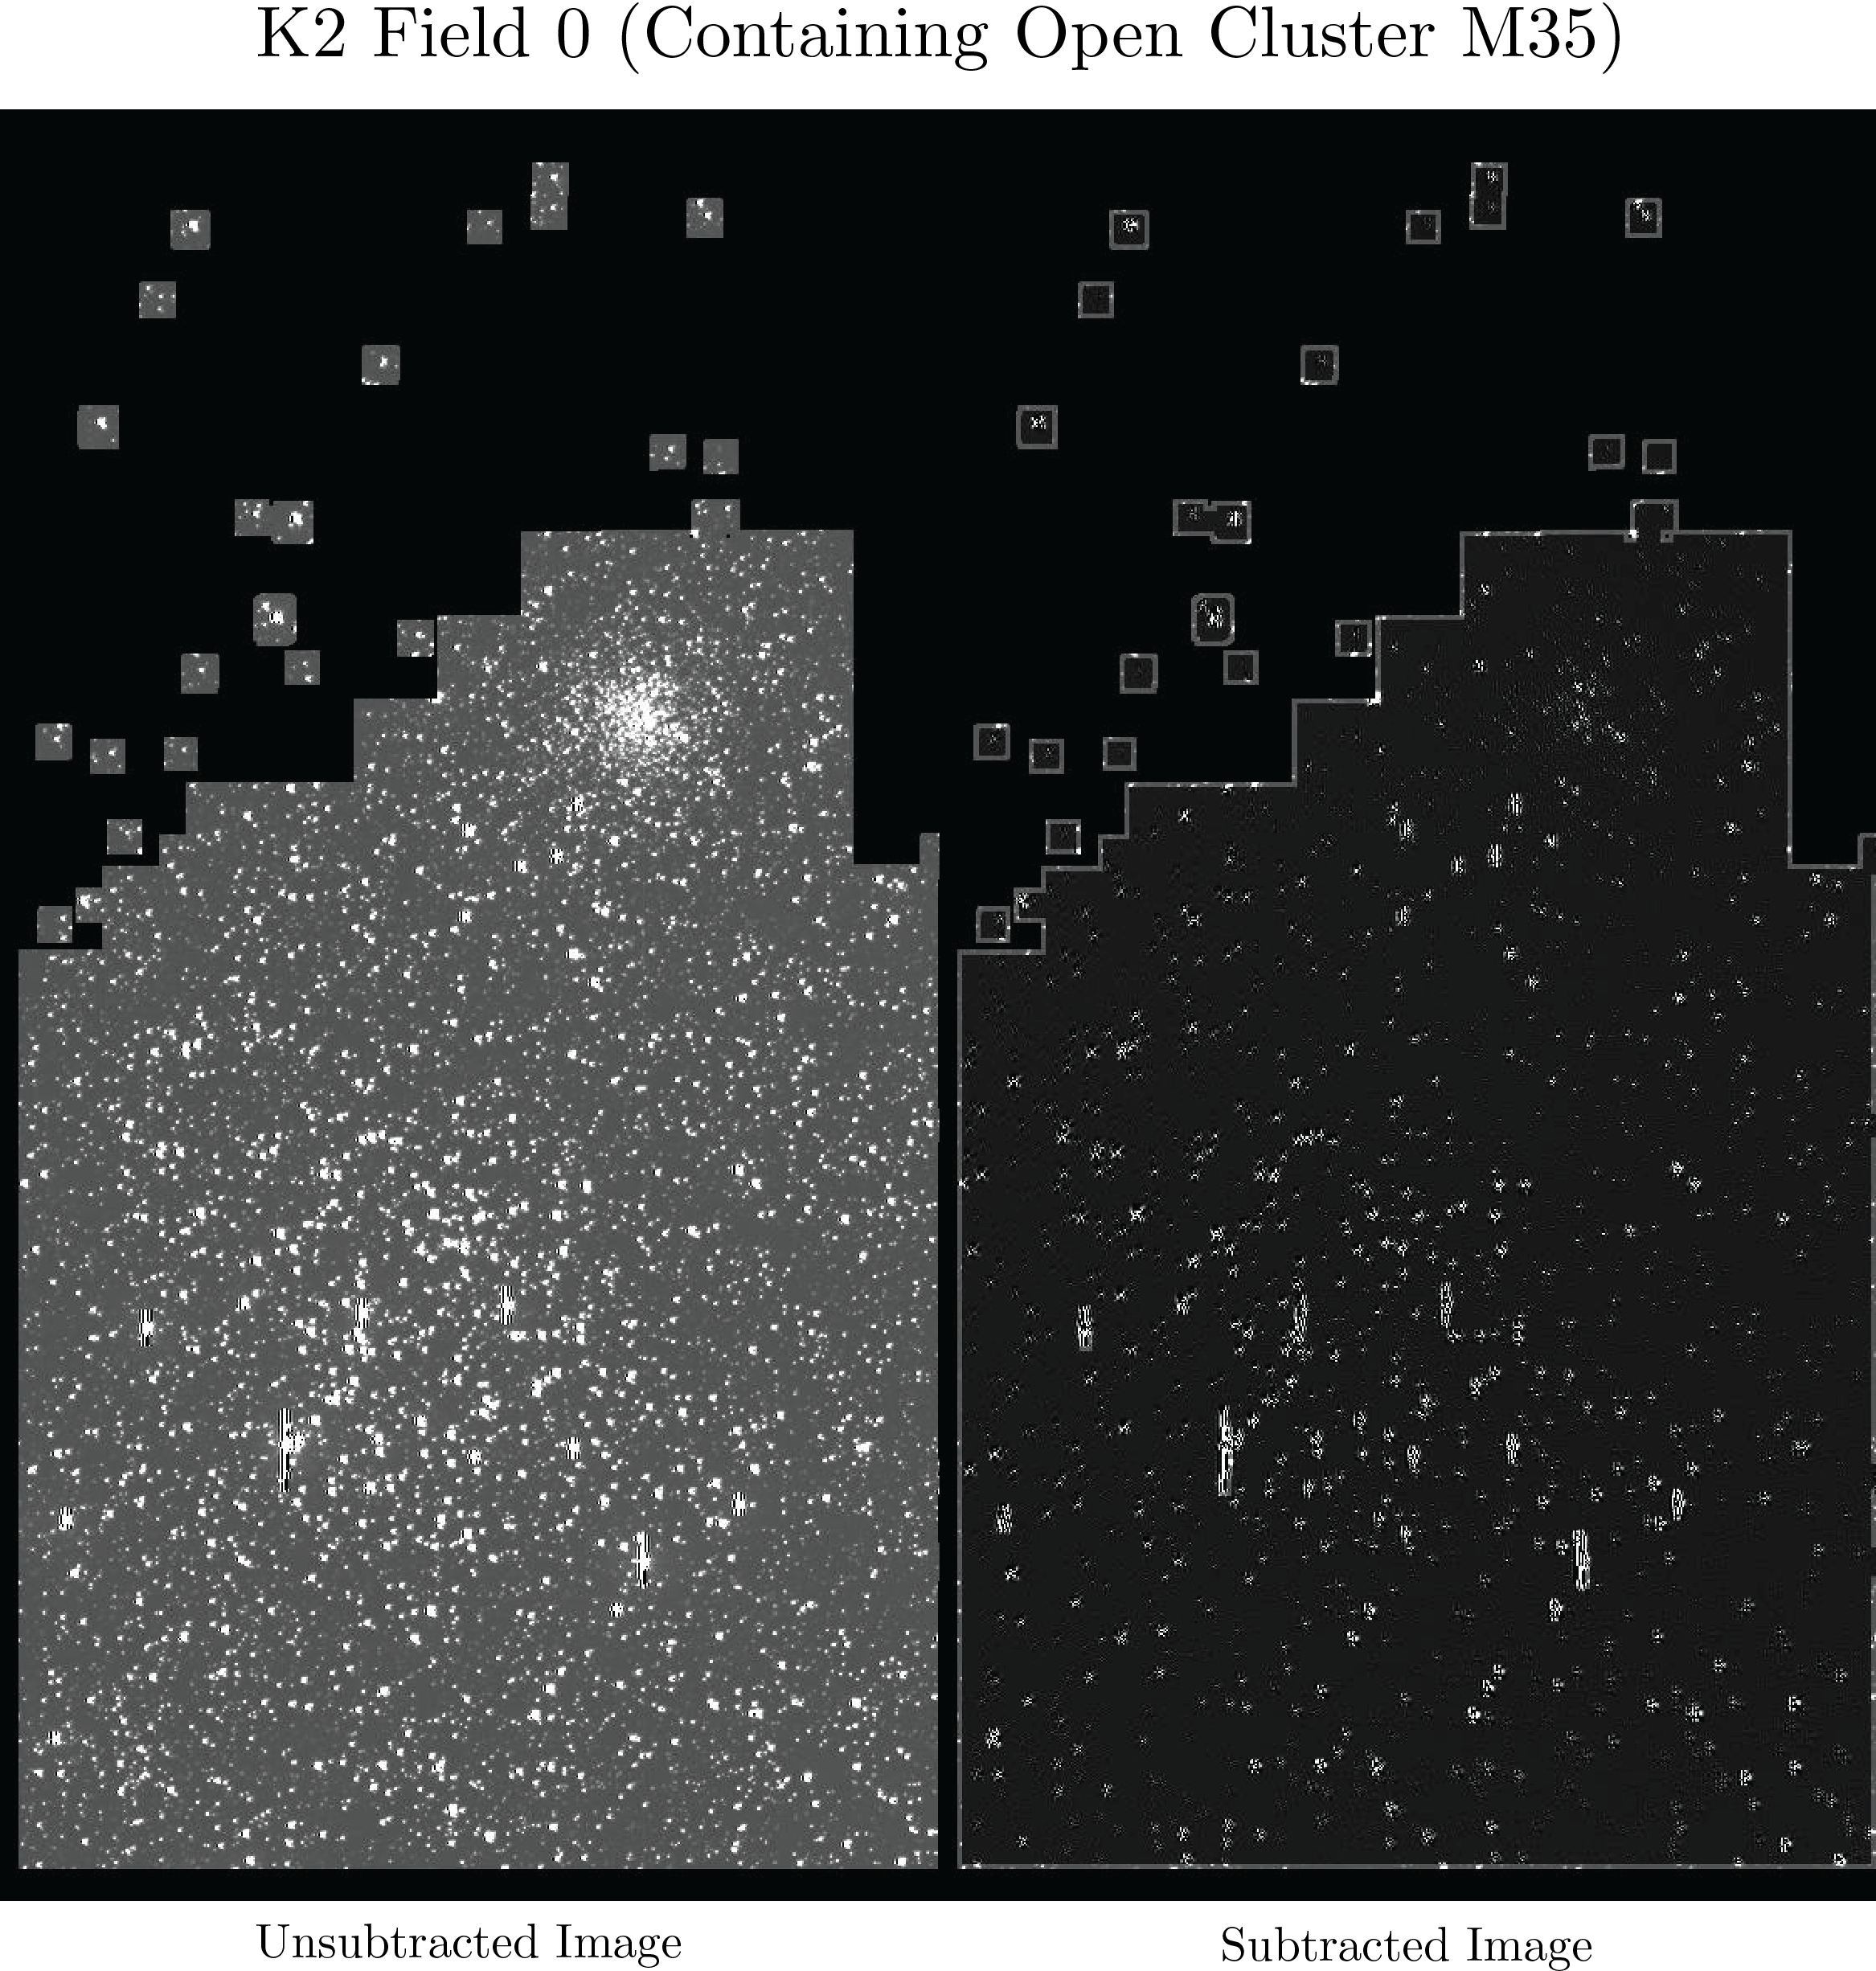
\includegraphics[width=0.8\textwidth]{Figure1Proposal.png}
\end{center}

The next task is to fine tune the parameters of the \textbf{melinda\_run\_ficonv.py} script. These parameters include \textbf{b}, \textbf{i}, \textbf{d} in the script. Joel claims I should start with nice low numbers, perhaps even 0! 

\subsection*{High Resolution Photref -- photometry with subtracted image}
Chelsea sent me an email with a helpful, in-depth description of the this step.\\  

Doing normal aperture photometry on the master image (i.e. the photometry reference), requires: 
\begin{enumerate}
\item \textbf{fiphot} - program used for aperture photometry
\item list of x,y coordinates for the stars we want to do photometry on 
\item fits image (photoref, with regions properly masked)
\item list of aperture to do the photometry on **start with a big list, making plots, and then choose the good few ones. 
\item method to convert magnitude to flux, I had a guess for Kepler, which is not too bad 
\end{enumerate}

All stars I query will have temporary HAT identifier numbers. 
After I release the light curve it will be linked to UCAC numbers.

The script that does the high-resolution photometry procedure is the shell script, \textbf{cmrawphot.sh}, however Chelsea recently wrote up a Python script for this bit.
The Python script is in the \textbf{chelseasrc} directory and is called \textbf{run\_iphot.py}. I renamed a version of this as \textbf{melinda\_run\_iphot.py}. I filled in the inputs referring to my past instruction and the \textbf{cmrawphot.sh} scripts and tested it on a few frames.\\ In order to work, I had to address a pickling error with a \textbf{copy\_reg module} workaround. It is now working fine, but it does take some time to run -- \textit{approximately 30 minutes or so}.

\subsubsection*{Getting list of x and y coordinates} 
\textit{How to get a list of x,y coordinates of stars?}\\
Chelsea already has this list compiled, so I can skip this bit. Here is the relevant background: \\
The file Chelsea made is called \textbf{photref.cat}
This is done by getting the astrometry solution on the photo ref/astro ref. 
Let's assume I have a file provided by Chelsea called \textbf{photref.trans}. 
This transfile is similar to the \textbf{itrans} file I used before, 
except it provides the polynomial transformation between 
$x_{i}$, $\eta$ $\rightarrow$ x,y (itrans provides the transformation between x,y $\rightarrow$ x,y). 
Usually this match has a worse result compared to the x,y$\rightarrow$x,y match.\\ 
Of course, for each of the stars, I only know about the RA and DEC.
$x_{i}$ and $\eta$ are obtained by calculating the distance of this star to a 
field center RA0 and DEC0, using a tangent transformation. 
So, there are two steps of transformation:
\begin{itemize}
\item RA and DEC $\rightarrow$  $x_{i}$ and $\eta$ (requires RA0 and DEC0) 
\item RA0 and DEC0 are read from the second to last line of the \textbf{transfile}.
\end{itemize}
\textcolor{red}{\textit{Review this above at a later time.}}\\ \\ 
The transformation itself is performed by calling: \\
\textbf{grtrans --input catfile --col-radec 2,3 --wcs 'tan,ra=rac,dec=dec,degrees' --col-out 5,6 --output outfile}\\ \\
$x_{i}$ and $\eta$ $\rightarrow$ RA and DEC (requires the transformation file)\\
\textbf{grtrans --input outfile (from above) --col-xy 5,6 -col-out 5,6 --input-transformation transfile --output starlistfile}

\subsubsection*{Photometry on Subtracted Frames}
This entire procedure is self-contained in the \textbf{melinda\_run\_iphot.py} script and therefore this bit can be ignored. 
This portion of the procedure actually performs photometry on the subtracted frames and uses the raw photometry from the master frame to infer the actual flux/magnitude of each stars on the non-subtracted frames. \\
This is done by calling the shell script, \textbf{IMG-3-PHOT\_M35.sh}.

Required to know:
\begin{itemize}
\item path for various files
\item raw photometry file
\item aperture list we used for raw photometry file
\item subtracted fits file
\end{itemize}
This script also requires the \textbf{itrans} file, the \textbf{JD} (or cadence or serial number) for each frame so later on I can generate light curves much easier. \\ \\
First the script calls the \textbf{fiphot} program in the subtracted frame photometry mode,then it transforms one sets of x,y coordinates back into the original frame coordinate using the \textbf{.itrans file}, and finally it prints out other relevant information that the light curve requires. \\ \\
 \textcolor{red}{\textit{Prints this ``relevant information'' in what format? Is this just the newly generated \textbf{.iphot} frames and the \textbf{photref\_M35.cmraw.phot} file?}}